\section{Приложение алгоритма случайного леса для классификации антропометрических данных}
\subsection{Предложенная модель} В работе используется модель Wrapper \cite{Vladimir2000} с целевой функцией для оценки алгоритма случайного леса, показанная на рисунке (рис. \ref{img19}).
\begin{figure}[ht!]
\centering
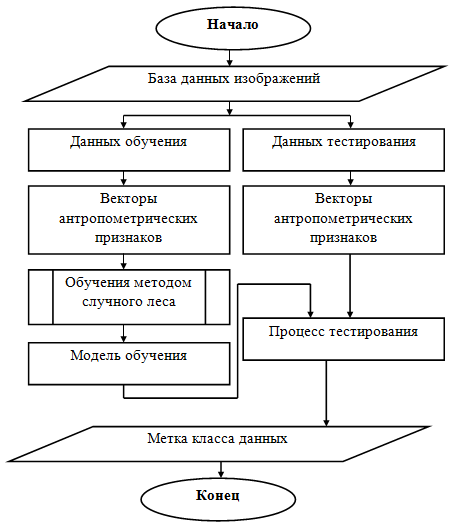
\includegraphics [scale=1] {images/h19.png}
\begin{center}
%\captionsetup{justification=justified, labelsep=period}
\caption{Предложенная модель} \label{img19}
\end{center}
\end{figure}
Архитектура системы состоит из двух основных частей. Часть $1$ используется, чтобы найти набор лучших атрибутов. Cистема генерирует наборы атрибутов, а затем использует алгоритм машинного обучения Random Forest для оценки таких наборов. Этот процесс повторяется до удовлетворения условий, чтобы остановить систему и получить набор оптимальных признаков. Часть $2$ используется, чтобы проверить подходит ли данная модель.
\subsection{Предложенный алгоритм}
В данной работе предлагается алгоритм случайного леса для классификации измерений для построения 3D модели на основе оценки и поиска набора антропометрических признаков из исходного набора признаков. Шаги выполнения алгоритма обозначается следующим образом:

\begin{itemize}
	\item \textbf{Шаг 1:} Создание $m$ наборов признаков из $n$ наборов первоначальных признаков. Каждый набор содержит $2 \frac{n}{m} $признаки. В том числе:
	
	\begin{itemize}
		\item  $\frac{n}{m}$ признаки равны;
		\item  $\frac{n}{m}$ случайные признаки.

	\end{itemize}
	
	\item \textbf{Шаг 2:} Использование Random Forest для того, чтобы вычислять оценку наборов признаков $\Rightarrow$ получение набора значений $f\left(i\right), i= \left(1,..., m\right)$;
	\item \textbf{Шаг 3:}взвешивание каждого признака $i$ рассчитывается по формуле:
	$w_j= \sum^m_{i=1}kf_i$;
	
	\begin{itemize}
		\item $k_{ij} = 0$, если признак $i$ не выбран в наборе признака $j$;
    \item $k_{ij}= 1$, если признак выбран в наборе признака $j$.
	\end{itemize}
	
	\item \textbf{Шаг 4:} Разработка нового признака включает в себя $р\%$ лучших признаков;
	\item \textbf{Шаг 5:} Повторение шага $1$ для удовлетворения одного из двух условий:
	
	\begin{itemize}
		\item Количество признаков < порога разрешено;
		\item Количество циклов определено.
	\end{itemize}
	
\end{itemize}

Изложенное выше направление рекомендуется для того, чтобы найти набор оптимальных маленьких признаков, таким образом, цель состоит в том, чтобы ограничить количество выходных признаков. Эти первоначальные признаки разделены для обеспечения всех выбранных признаков. Затем в сочетании с делением случайных признаков, создаются новые маленькие наборы признаков. Дальше алгоритм машинного обучения случайного леса используется для вычисления актуальности набора признаков. На основе значения расчетного уровня вычисления мы находим набор признаков, которые имеют меньшее количество свойств при сохранении целей работы.
\subsection{Формирование опорных точек с признаками объектной принадлежности}
В этом разделе представлен подход к реконструкции 3D-модели человека на основе антропометрических признаков, которые были извлечены и классифицированы из 2D-изображений. Мы используем набор данных  антропометрических признаков для построения 3D-модели точной и эффективной в соответствии с формой и фактическим размером объекта.

Процесс построения 3D-модели включает следующие шаги:

\begin{itemize}
	\item Шаг 1: Описание текстурных характеристик человеческого тела (кожа, волосы, лицо), а также текстуры одежды;
   \item Шаг 2: Разработка частей человеческого тела (голова, туловище, руки, ноги) с использованием ранее полученных антропометрических признаков;
\item Шаг 3: Комбинация текстуры и частей человеческого тела в блок;
\item Шаг 4: Экспорт антропометрических моделей человеческого тела в два файла: первый файл (*.mtl) описывает текстуры модели, второй файл (*.obj) содержает информацию каждой модели.
\end{itemize}

Алгоритм для соответствия 3D-модели с антропометрическими признаками:
\begin{figure}[ht!]
\centering
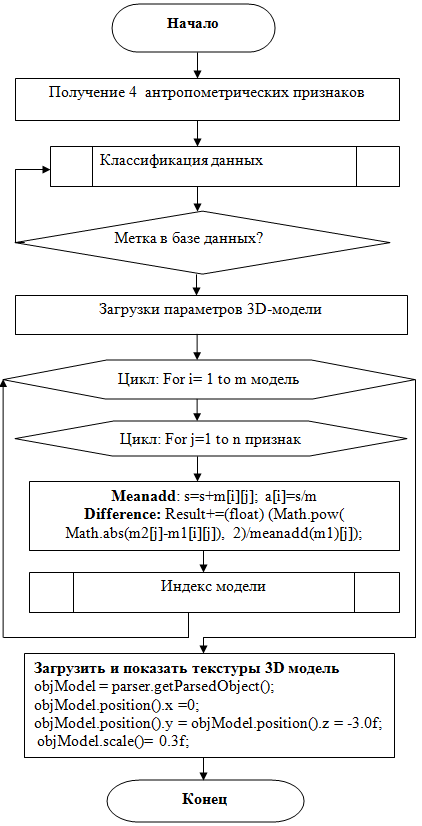
\includegraphics [scale=1] {images/h21.png}
\begin{center}
%\captionsetup{justification=justified, labelsep=period}
\caption{Алгоритм сопоставления 3D-формы с данными маркировки} \label{img21}
\end{center}
\end{figure}

\textbf{Результаты и анализ экспериментов на наборах антропометрических данных}

\textbf{Часть 1:} Обучение базового алгоритма случайного леса на наборах антропометрических данных выполнены $5$ раз с использоване библиотеки Weka \cite{Weka}. Каждый раз запуска будет диагонально выполнять проверки с количеством деревьев соответственно $100$, $200$, $300$, $400$, $500$ мы получим результат( в таблице \ref{tab5}):

\begin{table}[b!]%
\begin{center}
\caption{Результаты классификации на основе алгоритма случайного леса \cite{long1,long2}}\label{tab5}
  \begin{tabular}{|c|c|c|c|c|}
    \hline
 Количество  & Среднее   &   Стандартное   & Минимальное   & Максимальное \\
деревьев     & значение  &    отклонение   & значение      &значение      \\
\hline
100 &	0.03480	&0.025&	0.0139&	0.0606\\
\hline
200 &	0.02761	&0.0200	&0.0152	&0.0352\\
\hline
300	&0.02178	&0.0125	&0.0121	&0.0336\\
\hline
400	&0.01830	&0.0150	&0.0076	&0.0270\\
\hline
500	&0.01661	&0.0115	&0.0102	&0.0254\\
\hline

  \end{tabular}
\end{center}
\end{table}%\vspace{10mm}

\textbf{Часть 2:} Выбор набора оптимальных данных из наборов антропометрических данных мужчин первоначально предложенными методами выше. С начальным набором признаков, мы делим на m подразделение наборов признаков с использованием функции выборки <<$sample\left(, ,replace=True\right)$>> так что каждый набор содержит $\frac{n}{m}$ распределеные равномерные признаки и $\frac{n}{m}$ случайные признаки. Где $n$ - общее число признаков, $m$ - параметр распределения (в эксперименте выбрать $m=4$). В частности, файл результата <<ImportantFeature>> показывает новый набор, который включает в себя $4$ признака, расположенных соответственно в $12$ первоначальных признаках: $5,6,7,10$. С новым набором признаков, мы ещё раз выполняем часть $1$ представленную выше и получим результаты случайного леса при запуске пяти новых наборов признаков, показанных в таблице (\ref{tab6}).

\begin{table}[b!]%
\begin{center}
\caption{Результаты классификации на основе алгоритма случайного леса \cite{long1,long2}}\label{tab6}
  \begin{tabular}{|c|c|c|c|c|}
    \hline
  Количество  & Среднее   &   Стандартное   & Минимальное   & Максимальное \\
деревьев     & значение  &    отклонение   & значение      &значение      \\
\hline
100	&0.0116	&0.00833	&0.00463	&0.0202\\
\hline
200	&0.0092	&0.00667	&0.00516	&0.0117 \\
\hline
300	&0.02178	&0.00416	&0.0040	&0.0221\\
\hline
400	&0.00726	&0.0050	&0.0071	&0.009\\
\hline
500	&0.00553	&0.00383	&0.00513	&0.0085\\
\hline
  \end{tabular}
\end{center}
\end{table}%\vspace{10mm}

\subsubsection{Применение результатов классификации для построения 3D-моделей}
В работе \cite{grudinin2009} посвящена анализу антропометрических характеристик человеческого тела с целью определения границ изменения параметров и их взаимосвязи в рамках задачи параметрического моделирования компьютерных манекенов. В \cite{grudinin2014} предложен моделирование нестандартных параметризованных манекенов в рамках параметрического представления сложных геометрических объектов, удовлетворяющих заданным антропометрическим данным. Результаты исследований сосредоточены на построении частей человеческого тела: грудь и талию. Срок реализации 1-5 минут. В нашей работе используется результат классификации антропометрических данных, которые важные для построения антропологических моделей. При таком подходе, время работы программы быстрее и обеспечивает полную модель человеческого тела.

На основе выходных результатов процесса классификации - метка класса присваивается после процесса проверки. Основываясь на значении метки класса каждой записи, имеющееся $3D$-модель соответствует и подходит с параметрами каждой записи. $3D$-модели были построены при поддержке библиотек Min3D \cite{Min3D} и MakeHuman \cite{Make}. База данных включает в себя $100$ построенных моделей, в соответствии с размерами тела $XS$, $S$, $M$, $L$, $XL$. Каждый размер тела имеет $20$ моделей, построенных на основе каждого различного параметра тела.

На основе результата тестов, у нас имеется $5$ записей помеченых метками: $1$, $2$, $3$, $4$, $5$. Значит в очереди, записи имеют $3D$-модели соответствующие размерам $XS$, $S$, $M$, $L$, $XL$. Выбор наиболее подходящей модели для каждой записи будет основываться на $4$ признаках, которые выбраны из предлагаемого алгоритма: обхват груди $\left(B\right)$, обхват талии $\left(W\right)$, обхват бедер $\left(C\right)$, рост $\left(H\right)$. Мы создаем формулу для расчета следующим образом:
\begin{equation}\label{eq26}
Model = Min\left\{\sum^N_{i=1}\left(B-B_i\right)^2+\left(C-C_i\right)^2+\left(W-W_i\right)^2+\left(H-H_i\right)^2\right\}.
\end{equation}
Применение результатов алгоритма классификации случайного леса повышает точность результатов и уменьшает время вычисления в программе. График сравнения среднего времени при запуске случайного леса $5$ раз на новые наборы и начальные наборы антропометрических данных с количеством деревьев соответственно $100$, $200$,$300$, $400$, $500$ (рис. \ref{img20}).
\begin{figure}[ht!]
\centering
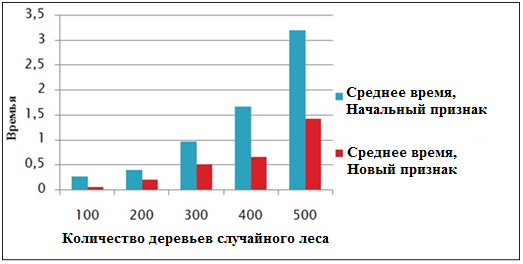
\includegraphics [scale=1] {images/h20.png}
\begin{center}
%\captionsetup{justification=justified, labelsep=period}
\caption{Время работы классификации для каждого набора данных.} \label{img20}
\end{center}
\end{figure}